\documentclass{beamer}
\usetheme{Cemef}


\usetheme{default} % You can change the theme as needed
\usepackage{array}
\usepackage{makecell}
\usepackage{subcaption}
\usepackage{parskip}
\usepackage[utf8]{inputenc}
\usepackage[T1]{fontenc}
\usepackage{amsmath}
\usepackage{amssymb}
\usepackage{algorithm}
\usepackage[noend]{algpseudocode}
\usepackage{float}
\usepackage{makecell}

\title{Statistical Methods}
\author{Samy Braik}
\date{\today}

\begin{document}

\begin{frame}
    \titlepage
\end{frame}

\section{Introduction}

\begin{frame}
    We denote by \(p\) the target distribution and \(q\) an easy-to-sample distribution, for example a centered Gaussian. The goal is to learn the distribution \(p\) ans sample from it.\\
\end{frame}

\begin{frame}{Diffusion}
    Let \(X_0\sim p\). We want to add noise until we reach pure noise, and denoise it afterward. We choose an horizon of time \(T\in\mathbb{N}^*\) and a noise schedule \(\beta:[0,T]\rightarrow\mathbb{R}^*\), continuous and non decreasing.

    \begin{block}{Forward process}
        \begin{align}
            d\overrightarrow{X}_t = \frac{-\beta(t)}{2\sigma^2}\overrightarrow{X}_t dt + \sqrt{\beta(t)}dB_t, \quad \overrightarrow{X}_0\sim p
        \end{align}
    \end{block}

    \begin{block}{Backward process}
        \begin{align}
            d\overleftarrow{X}_t=&\left(  \frac{\beta(T-t)}{2\sigma^2}\overleftarrow{X}_t+\beta(T-t)\nabla\log p_{T-t}\left(\overleftarrow{X}_t \right)  \right)dt \\ &+ \sqrt{\beta(T-t)}dB_t, \quad \overleftarrow{X}_0\sim p_T \nonumber
        \end{align}
            
    \end{block}
\end{frame}

\begin{frame}
    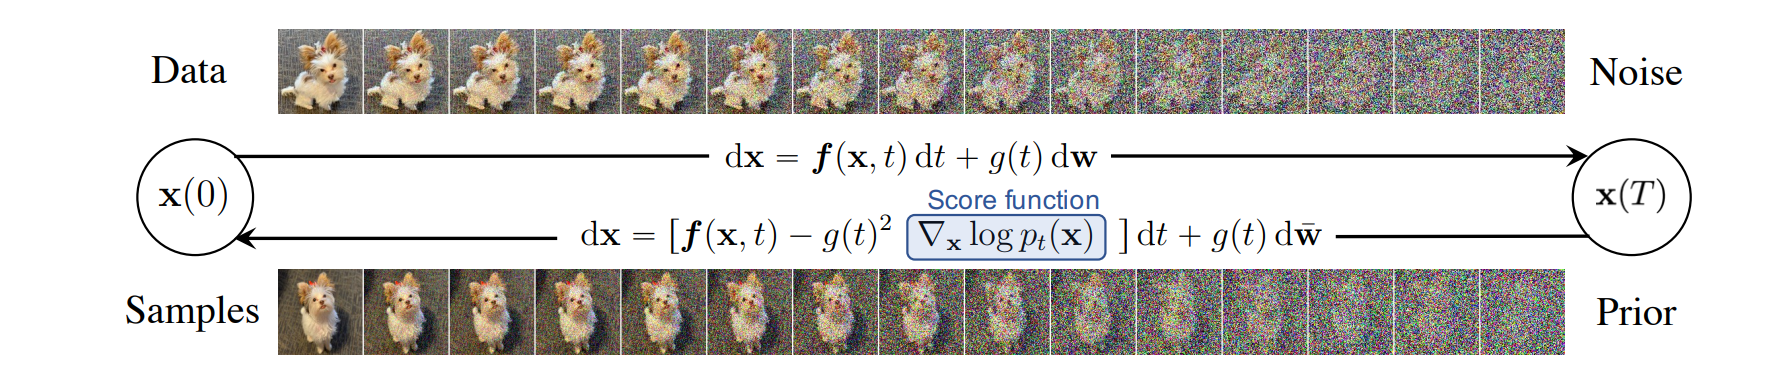
\includegraphics[width=1\linewidth]{score_based_dog.png}
    

    We learn the score by using score-matching techniques
    \begin{block}{Score matching}
        \begin{align}
            \mathcal{L}_\text{score}(\theta)=\mathbb{E}\left[ \left\| s_\theta \left(\tau,\overrightarrow{X}_\tau \right)-\log p_\tau \left(\overrightarrow{X}_\tau|X_0 \right)\right\|^2  \right]
        \end{align}
        where \(s_\theta\) is a neural network approximating the score function.
    \end{block}
    Plug it in the backward process and generate by discretizing the dynamics.
\end{frame}

\begin{frame}{Normalizing flow}
    Let \(x_0\sim q\) and \(f:\mathbb{R}^d\rightarrow\mathbb{R}^d\) an invertible and differentiable function an set  \(x_1:=f(x_0)\) such that \(x_1\sim p\).\\
    We can write the density \(p\) as
    \begin{align}
        p(x_1) &= q(f^{-1}(x_1))\left| \det \frac{\partial f^{-1}}{\partial x_1}(x_1)\right|\\
        &= q(f^{-1}(x_1))\left| \det \frac{\partial f}{\partial x_0}(f^{-1}(x_1))\right|^{-1} 
    \end{align}
    We can then write the log-likelihood as
    \begin{align}
        \log p(x_1) &= \log p(f^{-1}(x_1))-\log \left| \det \frac{\partial f}{\partial x_0}(f^{-1}(x_1))\right|
    \end{align}
\end{frame}

\begin{frame}{Normalizing flow}
    Let \(X_0\sim q\) and \(X_1\sim p\). We want to learn \(f_\theta\) such that \(X_1 \simeq f_\theta(X_0)=Z\sim p_Z\). To do that, we set a structure on \(f_\theta\), with \(\phi_1,\ldots,\phi_k\) simpler function (all parametrized by \(\theta\)) such that 
    \[f_\theta=\phi_k\circ\ldots\circ \phi_1\] 
    We determine \(f_\theta\) by minimizing 
    \[\mathcal{L}_\text{NF}(\theta)= \mathbb{E}\left[-\log p_Z(f_\theta(x))-\log \left|\det \frac{\partial f_\theta}{\partial x}(x)\right|\right]\]
\end{frame}

\begin{frame}{Normalizing flow}
    An early instances  of normalizing flow is the planar flow 
    \begin{align*}
        \phi_k(x)=x+\sigma(b_k^\intercal x+c)a_k
    \end{align*}
    where \(a_k,b_k\in\mathbb{R}^d, c\in\mathbb{R}\) and  \(\sigma:\mathbb{R}\rightarrow\mathbb{R}\) is a non-linear function.
\end{frame}

\begin{frame}{Flow matching}
    We start by defining a probability density path
    \begin{block}{Probability density path}
        A probability path \(p:[0,1]\times\mathbb{R}^d\rightarrow\mathbb{R}^d\) meaning that for each time \(t\), \(p_t\) is density function i.e. \(\int p_t(x)dx=1\).\\
    \end{block}
    A simple example of such a path is a path \(p\) interpolating two density \(p_0\) and \(p_1\) with \(p_t=tp_1+(1-t)p_0\)
    \begin{figure}[htbp]
        \centering
        \caption{A probability path interpolating $\mathcal{N}(0,0.2)$ and $\mathcal{U}([0,1])$}
    \end{figure}
\end{frame}


\begin{frame}
    \begin{figure}[h]
        \centering
        \begin{subfigure}[b]{0.8\textwidth}
          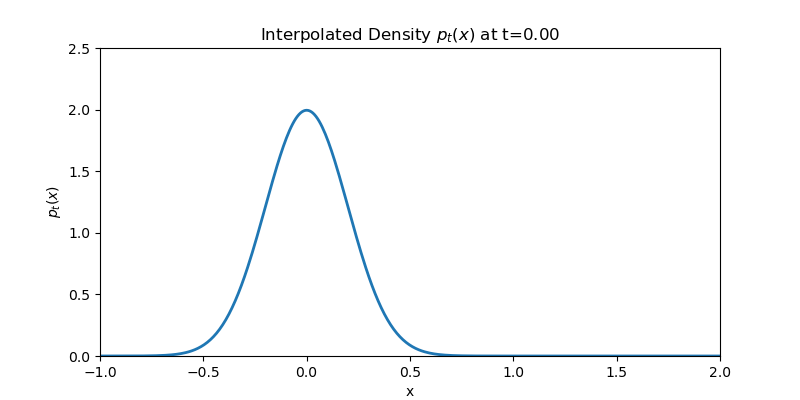
\includegraphics[width=\linewidth]{/home/admin-sbraik/Documents/InternshipProduction/FlowMatching/frames/frame_1.png}
        \end{subfigure}
        \par\medskip
        \begin{subfigure}[b]{0.8\textwidth}
          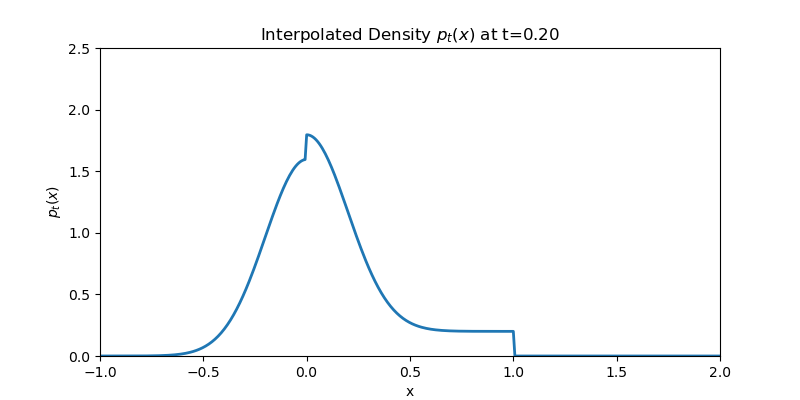
\includegraphics[width=\linewidth]{/home/admin-sbraik/Documents/InternshipProduction/FlowMatching/frames/frame_2.png}
        \end{subfigure}
    \end{figure}

\end{frame}

\begin{frame}
    \begin{figure}[htbp]
        \centering
        \begin{subfigure}[b]{0.8\textwidth}
          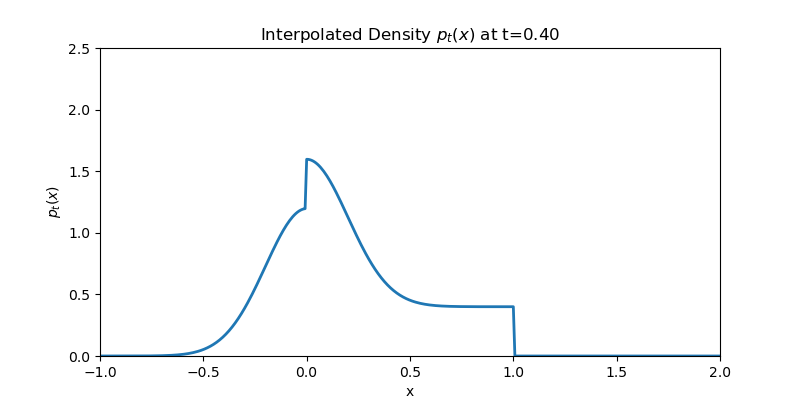
\includegraphics[width=\linewidth]{/home/admin-sbraik/Documents/InternshipProduction/FlowMatching/frames/frame_3.png}
        \end{subfigure}
        \par\medskip
        \begin{subfigure}[b]{0.8\textwidth}
          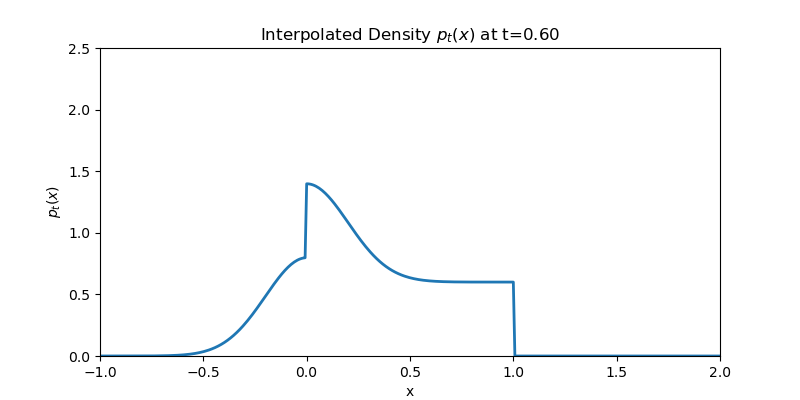
\includegraphics[width=\linewidth]{/home/admin-sbraik/Documents/InternshipProduction/FlowMatching/frames/frame_4.png}
        \end{subfigure}
    \end{figure}
\end{frame}
\begin{frame}
    \begin{figure}[htbp]
        \centering
        \begin{subfigure}[b]{0.8\textwidth}
          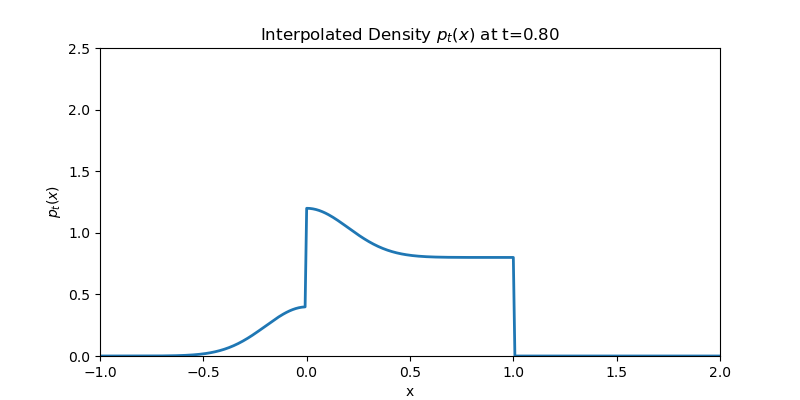
\includegraphics[width=\linewidth]{/home/admin-sbraik/Documents/InternshipProduction/FlowMatching/frames/frame_5.png}
        \end{subfigure}
        \par\medskip
        \begin{subfigure}[b]{0.8\textwidth}
          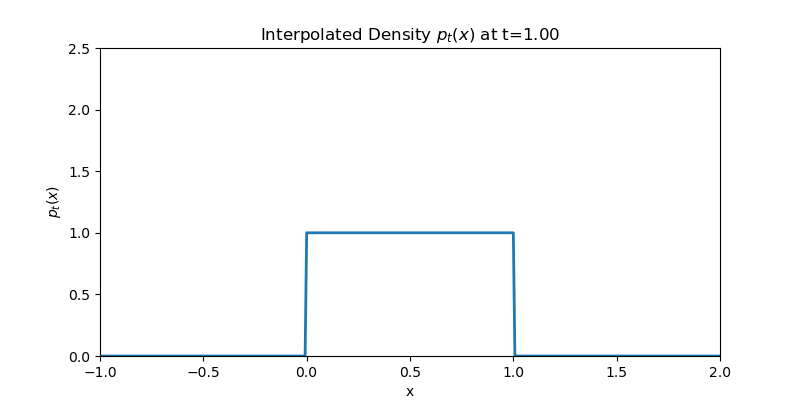
\includegraphics[width=\linewidth]{/home/admin-sbraik/Documents/InternshipProduction/FlowMatching/frames/frame_6.png}
        \end{subfigure}
        
        \label{fig:interpolated_density}
    \end{figure}
\end{frame}


\begin{frame}{Flow matching}
    Next we introduce a core object, a time dependent vector field \(v:[0,1]\times\mathbb{R}^d\rightarrow \mathbb{R}^d\) which is used to construct a map \(\phi:[0,1]\times\mathbb{R}^d\rightarrow\mathbb{R}^d\), called a flow, by the following ODE
    \begin{align}
        \frac{d}{dt}\phi_t(x)&=v_t(\phi_t(x)) \\
        \phi_0(x)&=x \nonumber
    \end{align}
    The link between the flow and the probability path is given by the change of variable formula
    \begin{align}
        p_t(x)=q(\phi_t^{-1}(x))\det \left[\frac{\partial\phi_t^{-1}}{\partial x}(x)\right]
    \end{align}
    That coincides with the normalizing flow case.
\end{frame}

\begin{frame}
    The link between the vector field and the probability path is given by the continuity equation 
    \begin{align}
        \frac{d}{dt}p_t(x)+\text{div}\left[v_t(x)p_t(x)\right]=0
    \end{align}
    It said that the vector field \(v_t\) generates the probability path \(p_t\) if it satisfies the continuity equation.\\

    \begin{figure}[b]
        \centering
        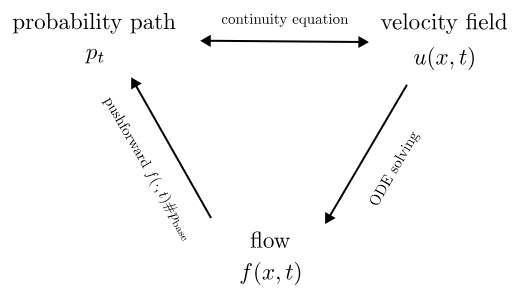
\includegraphics[width=0.7\linewidth]{images/LinkBetweenObjects.png}
        \caption{Link between marginal flow matching objects}
        \label{fig:flow_matching}
    \end{figure}
\end{frame}

\begin{frame}{Flow matching}
    Given a probability path \(p_t\) and a vector field \(v_t\), the naïve flow matching loss is defined by
    \begin{align}
        \mathcal{L}_\text{FM}(\theta)=\mathbb{E}_{t,p_t(x)}\left[ \| v_t^\theta(x)-v_t(x)\|^2 \right]
    \end{align}
    but we don't have acces to \(v_t\) and \(p_t\).
    \bigskip
    To adress this problem, we introduce new objects. 
\end{frame}

\begin{frame}{Flow matching}
    Given a particular data sample \(x_1\) from \(p\), we introduce a conditional probability path \(p_t(x|x_1)\) such that at time \(t=0\) \(p_0(x|x_1)=q(x)\) and by marginalizing over \(x_1\) we can recover the marginal probability path 
    \begin{align}
        p_t(x)=\int p_t(x|x_1)p(x_1)dx_1
    \end{align}
    Instead of working with a probability density, we consider samples from our distributions and define how to go from one to the other.\\
\end{frame}
    
\begin{frame}{Flow matching}
    In the same vein, we can define a conditional vector field, assuming \(p_t(x)>0\) for all \(t\) and \(x\)
    \begin{align}
        v_t(x)=\int v_t(x|x_1)\frac{p_t(x|x_1)p(x_1)}{p_t(x)}dx_1
    \end{align}
\end{frame}

\begin{frame}
\begin{figure}
    \centering
    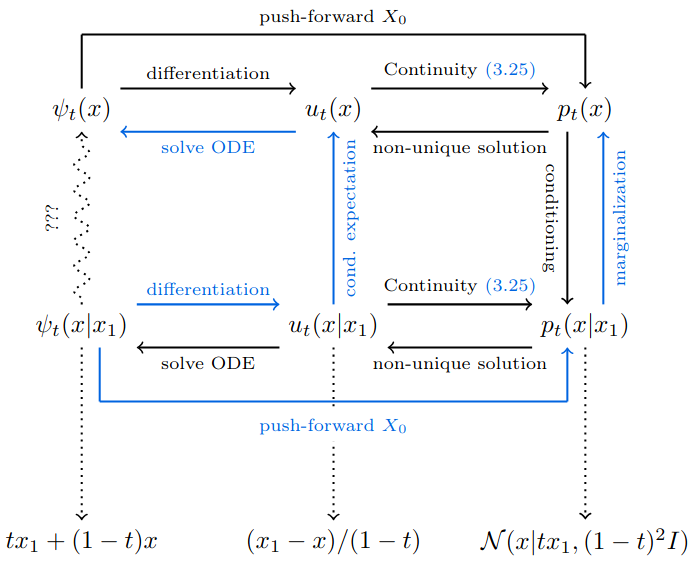
\includegraphics[width=0.9\linewidth]{/home/admin-sbraik/Documents/InternshipProduction/FlowMatching/FlowMatchingFramework.png}
    \caption{Link between all the flow matching objects}
    \label{fig:flow_matching_full}
\end{figure}
\end{frame}

\begin{frame}{Flow matching}
    The new loss function, called conditional flow mathcing loss, is defined as
    \begin{align}
        \mathcal{L}_\text{CFM}(\theta)=\mathbb{E}_{t,p_t(x|x_1)}\left[ \| v_t^\theta(x|x_1)-v_t(x|x_1)\|^2 \right]
    \end{align}
    with the property : \( \mathcal{L}_\text{FM}(\theta)=\mathcal{L}_\text{CFM}(\theta) \) up to a constant independant of \(\theta\).
\end{frame}


\begin{frame}{Flow matching}
    With in mind 
    \begin{align*}
        v_t(x|x_1),p_t(x|x_1)\iff \phi_t(x|x_1)
    \end{align*}
    \begin{algorithm}[H]
        \caption{Flow matching training}\label{alg:flow_matching_training}
            \begin{algorithmic}
                \State \textbf{Input:} dataset \(p\), noise \(q\)
                \State Initialized \(v^\theta\)
                \While{not converged}
                    \State \(t\sim\mathcal{U}([0,1])\)
                    \State \(x_1\sim p(x_1)\)
                    \State \(x_0\sim q(x_0)\)
                    \State \(x_t=\phi_t(x_0|x_1)\)
                    \State Gradient step with \(\nabla_\theta \| v_t^\theta (x_t) -\dot{x}_t \|^2\)
                \EndWhile
                \State \textbf{Output:} \(v^\theta\)
            \end{algorithmic}
        \end{algorithm}
\end{frame}

\begin{frame}{Flow matching}
    \begin{algorithm}[H]
        \caption{Flow matching sampling}\label{alg:flow_matching_sampling}
            \begin{algorithmic}
                \State \textbf{Input:} Trained \(v^\theta\)
                \State \(x_0\sim q(x_0)\)
                \State Solve numerically the ODE \(\dot{x}_t=v_t^\theta(x_t)\)
                \State \textbf{Output:} \(x_1\)
            \end{algorithmic}
    \end{algorithm}
\end{frame}

\begin{frame}{Choice of conditional flow}
    \begin{block}{Linear flow}
        The simplest flow is a linear flow defined by
        \begin{align}
            \phi_t(x|x_1)=\alpha_t x+\sigma_t x_1
        \end{align}
        where \(\alpha_t\) and \(\sigma_t\) are two differentiable functions and satisfy the constraint \(\alpha_0=\sigma_1=1\) and \(\alpha_1=\sigma_0=0\).

        \bigskip
        In particular, the simplest setting is to choose \(\alpha_t=1-t \) and \(\sigma_t=t\). This is called the \textbf{rectified flow}.
    \end{block}
\end{frame}

\begin{frame}{Link between diffusion and flow matching}
    \begin{block}{Gaussian flow}

        
    \end{block}
\end{frame}

\begin{frame}{Link between normalizing flow and flow matching}
    When considering a transformation \(\phi(x)=x+\frac{1}{K}v(x)\) in the normalizing flow context, we can re-arrange the equation to obtain
    \begin{align*}
        \frac{\phi(x)-x}{1/K}=v(x)
    \end{align*}
    Taking the limit \(K\rightarrow \infty\) gives us the ODE
    \begin{align*}
        \frac{dx_t}{d}=\lim_{K\rightarrow \infty}\frac{x_{t+1/K}-x_t}{1/K}=\frac{\phi_t(x_t)-x_t}{1/K}=v_t(x_t)
    \end{align*} 
    where the flow \( \phi:[0,1]\times\mathbb{R}^d\rightarrow\mathbb{R}^d\) is defined by the ODE
    \begin{align*}
        \frac{d\phi_t}{d}=v_t(\phi_t(x_0))
    \end{align*}
\end{frame}

\begin{frame}{Comparison}
    %\hspace*{-1cm} % Remove left indentation
    \scalebox{0.8}{
    \begin{tabular}{|c|c|c|}
        \hline
        Models & Pros & Cons \\
        \hline
        Diffusion & \makecell{Easy to train} & \makecell{Hard to sample (solve a SDE) \\Only works with Gaussian} \\
        Normalizing flow & \makecell{Exact density estimation} & \makecell{Computationally intensive \\Not expressive} \\ 
        Flow matching & \makecell{Exact density estimation \\ Simulation free training \\Easy to sample}  & \makecell{test}\\
        Kernel estimator & \makecell{Flexible Easy to exploit}  & \makecell{Slow rate of convergence \\ Hard to evaluate at new data point \\ Hard to choose tuning parameters \\ Need a lot of data}\\
        \hline
    \end{tabular}
    }
\end{frame}



\end{document}